\chapter{Dynamics}
\begin{itemize}
    \item \emph{Newton's First Law of Motion} states that an object at rest will remain at rest and an object in motion will remain in motion at constant velocity in a straight line in the absence of an \emph{external} resultant force.
    \item The \emph{linear momentum} of a body is the product of its mass and velocity. The linear momentum is in the \emph{same direction} as its velocity.
    \item \emph{Newton's Second Law of Motion} states that the rate of change of momentum of a body is directly proportional to the resultant force acting on the body and occurs \emph{in the direction} of the resultant force.
    \item \emph{Newton's Third Law of Motion} states that if body A exerts a force on body B, then body B exerts a force of the \emph{same type} that is equal in magnitude and opposite in direction on body A.
    \item \emph{Impulse} is defined as the product of \emph{average} force acting on an object and the time for which the force acts.
    \item The \emph{Principle of Conservation of Linear Momentum} states that the total momentum of a system remains constant provided no \emph{external} resultant force acts on the system. i.e.
    \[m_1u_1+m_2u_2=m_1v_1+m_2v_2.\]
    \item A elastic collision is on where kinetic energy is conserved. i.e.
    \[m_1u_1^2+m_2u_2^2=m_1v_1^2+m_2v_2^2.\]
    \item The below table provides a quick shortcut, that is particularly helpful in solving multiple choice questions fast. We assume a mass \(m_1\) is moving with velocity \(u\) towards a \emph{stationary} (\(u_2=0\)) mass \(m_2\).
    \begin{table}[H]
        \centering
        \begin{tabular}{ScScSc}
            \toprule 
            Case & \(v_1\) & \(v_2\)\\
            \midrule
            \(m_1=m_2\) & \(0\) & \(u\)\\
            \(m_1\ll m_2\) & \(\approx -u\) & \(\approx 0\)\\
            \(m_1\gg m_2\) & \(\approx u\) & \(\approx 2u\)\\
            \bottomrule
        \end{tabular}
        \caption{Special cases of elastic collisions.}
        \label{table:elastic-collisions}
    \end{table}
    \item For an elastic collision, the relative speed of approach is equal to the relative speed after collision:
    \[u_1\highlight[green!50]{-u_2}=v_2\highlight[green!50]{-v_1}.\]
    \emph{Note.} The formula is \textcolor{red}{\emph{not} \(u_1-u_2=v_1-v_2\)}.
    \item An inelastic collision is one where kinetic energy is not conserved. 
    \item In a perfectly inelastic collision, the masses coalesce (become one) and move off with the same velocity. In other words,
    \[m_1u_1+m_2u_2=(m_1+m_2)v.\]
\end{itemize}
\begin{figure}[H]
    \centering
    \begin{subfigure}[c]{\textwidth}
        \centering
        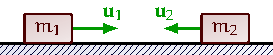
\includegraphics[page=1]{../images/collisions/collisions.pdf}
        \caption{The masses travelling towards each other, before colliding.}
    \end{subfigure}%

    \vspace{1em}
    \begin{subfigure}[c]{0.4\textwidth}
        \centering
        \includegraphics[page=2]{../images/collisions/collisions.pdf}
        \caption{After an elastic collision, the masses may travel in opposite directions.}
    \end{subfigure}\hfill
    \begin{subfigure}[c]{0.5\textwidth}
        \centering
        \includegraphics[page=3]{../images/collisions/collisions.pdf}
        \caption{After an elastic collision, the masses may travel in the same direction.}
    \end{subfigure}%

    \vspace{1em}
    \begin{subfigure}[c]{\textwidth}
        \centering
        \includegraphics[page=4]{../images/collisions/collisions.pdf}
        \caption{After an inelastic collision, the coalesced masses travel together in the same direction, with equal velocities.}
    \end{subfigure}%
    \caption{\ref{source:collision} An illustration of (perfectly) elastic and inelastic collisions.}
    \label{fig:collision-1d}
\end{figure}
\begin{figure}[H]
    \centering
    \includegraphics[page=7]{../images/collisions/collisions.pdf}
    \caption{\ref{source:collision} Another illustration of a (perfectly) inelastic collision.}
    \label{fig:collision-2d}
\end{figure}
\begin{itemize}
    \item An explosion does not conserve kinetic energy. But momentum is still conserved. Suppose a (stationary) mass splits into \(n\) masses \(m_1\), \(m_2\), \dots, \(m_n\). Then we have
    \[m_1v_1+m_2v_2+\dots+m_nv_n=0.\]
\end{itemize}
\chapter{Forces}
\begin{center}
    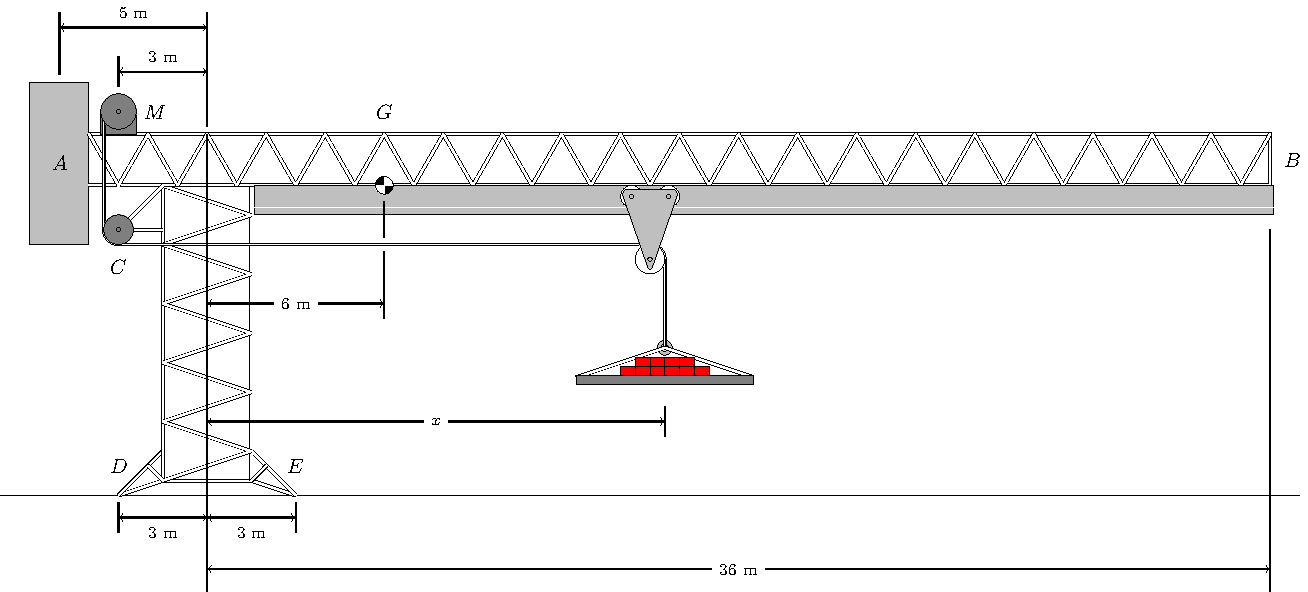
\includegraphics[width=\textwidth,page=1]{../images/Crane/Crane.pdf}
    \captionsetup{type=figure}
    \caption[figure]{\ref{Crane} Forces acting on a crane.}
\end{center}
\begin{figure}[H]
    \centering
    \includegraphics[page=2]{../images/ladder/ladder.pdf}
    \caption{\ref{source:fbd-ladder} The free body diagram for a ladder, on which a person stands, and which is leaning against a wall.}
    \label{fig:fbd-ladder}
\end{figure}
\begin{itemize}
    \item A field of force due to a body's property (e.g. charge, mass) is a region in space in which a body carrying that property experiences a force when it is placed in the field.
    \item \emph{Hooke's Law} states that the force acting on a material directly proportional to the extension in the material, provided that the \emph{limit of proportionality} is not exceeded.
    \item The \emph{center of gravity} of an object is the point at which the entire weight of a body may be considered to act.
    \item For a mass placed on a ramp, the forces it experiences are as shown below.
    \begin{figure}[H]
        \centering
        \begin{subfigure}[c]{0.3\textwidth}
            \centering
            \includegraphics[page=4]{../images/Force-Triangle/Force-Triangle.pdf}
        \end{subfigure}%
        \begin{subfigure}[c]{0.3\textwidth}
            \centering
            \includegraphics[page=5]{../images/Force-Triangle/Force-Triangle.pdf}
        \end{subfigure}%
        \caption{\ref{source:forces-triangle} Mass \(m\) placed on a ramp whose top surface makes an angle \(\theta\) with the horizontal.}
        \label{fig:forces-triangle}
    \end{figure}
    \item The \emph{moment} of a force is equal to the product of the force and the \emph{perpendicular} distance of the \emph{line of action} of the force from the pivot. It is also the turning effect of a force.
    \item \emph{Torque of a couple} is defined as the product of one of the forces and the \emph{perpendicular} distance between the \emph{lines of action} of the forces.
    \begin{figure}[H]
        \centering
        \begin{subfigure}[c]{0.3\textwidth}
            \centering
            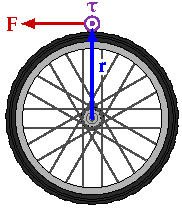
\includegraphics[page=1]{../images/torque/torque.pdf}
            \caption{A perpendicular force.}
        \end{subfigure}%
        \begin{subfigure}[c]{0.3\textwidth}
            \centering
            \includegraphics[page=2]{../images/torque/torque.pdf}
            \caption{A parallel force.}
        \end{subfigure}%
        \begin{subfigure}[c]{0.3\textwidth}
            \centering
            \includegraphics[page=3]{../images/torque/torque.pdf}
            \caption{A force which is neither perpendicular nor parallel.}
        \end{subfigure}%
        \caption{\ref{source:torque} The torque of a force acting on a wheel}
        \label{fig:torque-wheel}
    \end{figure}
    \item The \emph{Principle of Moments} states that if a body is in rotational equilibrium, the (vector) sum of all the clockwise moments about \emph{any axis} must be equal in magnitude to the (vector) sum of anticlockwise moments about the \emph{same axis}.
    \begin{figure}[H]
        \centering
        \includegraphics[page=4]{../images/torque/torque.pdf}
        \caption{\ref{source:torque} The free body diagram of a lever, which is in equilibrium iff \(m_1gr_1=m_2gr_2\).}
        \label{fig:torque-lever}
    \end{figure}
    \item \emph{Note.} When using the Principle of Moments, always make clear which pivot/axis of rotation is being considered. E.g. ``Taking moments about \rule{0.5cm}{0.01mm}, by the principle of moments, \dots''
    \item \emph{Density} is defined as the mass per unit volume of a substance.
    \item \emph{Pressure} is defined as force per unit area, where the force is \emph{acting perpendicularly} to the area.
\end{itemize}
\begin{minipage}{0.3\textwidth}
    \begin{figure}[H]
        \centering
        \includegraphics[page=5]{../images/pressure/pressure.pdf}
        \caption{\ref{source:pascal's-law} A column of fluid.}
        \label{fig:pascal's-law}
    \end{figure}
\end{minipage}%
\begin{minipage}{0.7\textwidth}
    \begin{itemize}
        \item Deriving \(p=\rho gh\):
        \begin{enumerate}
            \item Consider a point at a depth \(h\) below the surface of a liquid of density \(\rho\). 
            \item The force \(F\) acting perpendicularly on a surface area \(A\) at depth \(h\) is due to the weight of the liquid column above \(A\) to give pressure \(p\). Thus, \(p=\frac{F}{A}=\frac{mg}{A}=\frac{\rho Ah}{g}=\rho gh\).
        \end{enumerate}
    \end{itemize}
\end{minipage}
\begin{itemize}
    \item \emph{Upthrust} is the upward force exerted by a fluid on a body immersed in the fluid (due to pressure difference in the fluid).
    \item \emph{The origin of upthrust:} Upthrust is a result of the pressure difference between top and bottom surfaces of the body, resulting in a net upwards force being exerted on the body by the third medium in which the body is located.
\end{itemize}
\begin{minipage}{0.5\textwidth}
    \begin{figure}[H]
        \centering
        \begin{subfigure}[c]{0.5\textwidth}
            \centering
            \includegraphics[page=3]{../images/Upthrust/Upthrust.pdf}
        \end{subfigure}%
        \begin{subfigure}[c]{0.5\textwidth}
            \centering
            \vspace{1cm}
            \includegraphics[page=4]{../images/Upthrust/Upthrust.pdf}
        \end{subfigure}%
        \caption{\ref{source:archimedes-principle} An illustration of Archimedes' Principle.}
        \label{fig:archimedes-principle}
    \end{figure}
\end{minipage}%
\begin{minipage}{0.5\textwidth}
    \begin{itemize}
        \item \emph{Archimedes' Principle} states that when a body is totally or partially immersed in a fluid, it experiences an upward force (upthrust) equal to the weight of fluid displaced.
        \item \emph{The Principle of Floatation} states that, for any object floating in \emph{equilibrium}, the upthrust is equal to the weight of the object.
    \end{itemize}
\end{minipage}
\begin{itemize}
    \item Remember to account for atmospheric pressure, where necessary.
    \item Suppose a body is subjected to forces acting at three points. Then, for it to be in equilibrium, the lines of action must be \emph{concurrent} (intersection at a common point) or \emph{parallel}. 
\end{itemize}
\begin{example}{}{}
    A uniform strip of steel is clamped at one end. A metal block of mass \(M\) is fixed to the strip, a distance \(L\) from the clamp. The mass causes the end of the steel strip to be depressed.
    \begin{figure}[H]
        \centering
        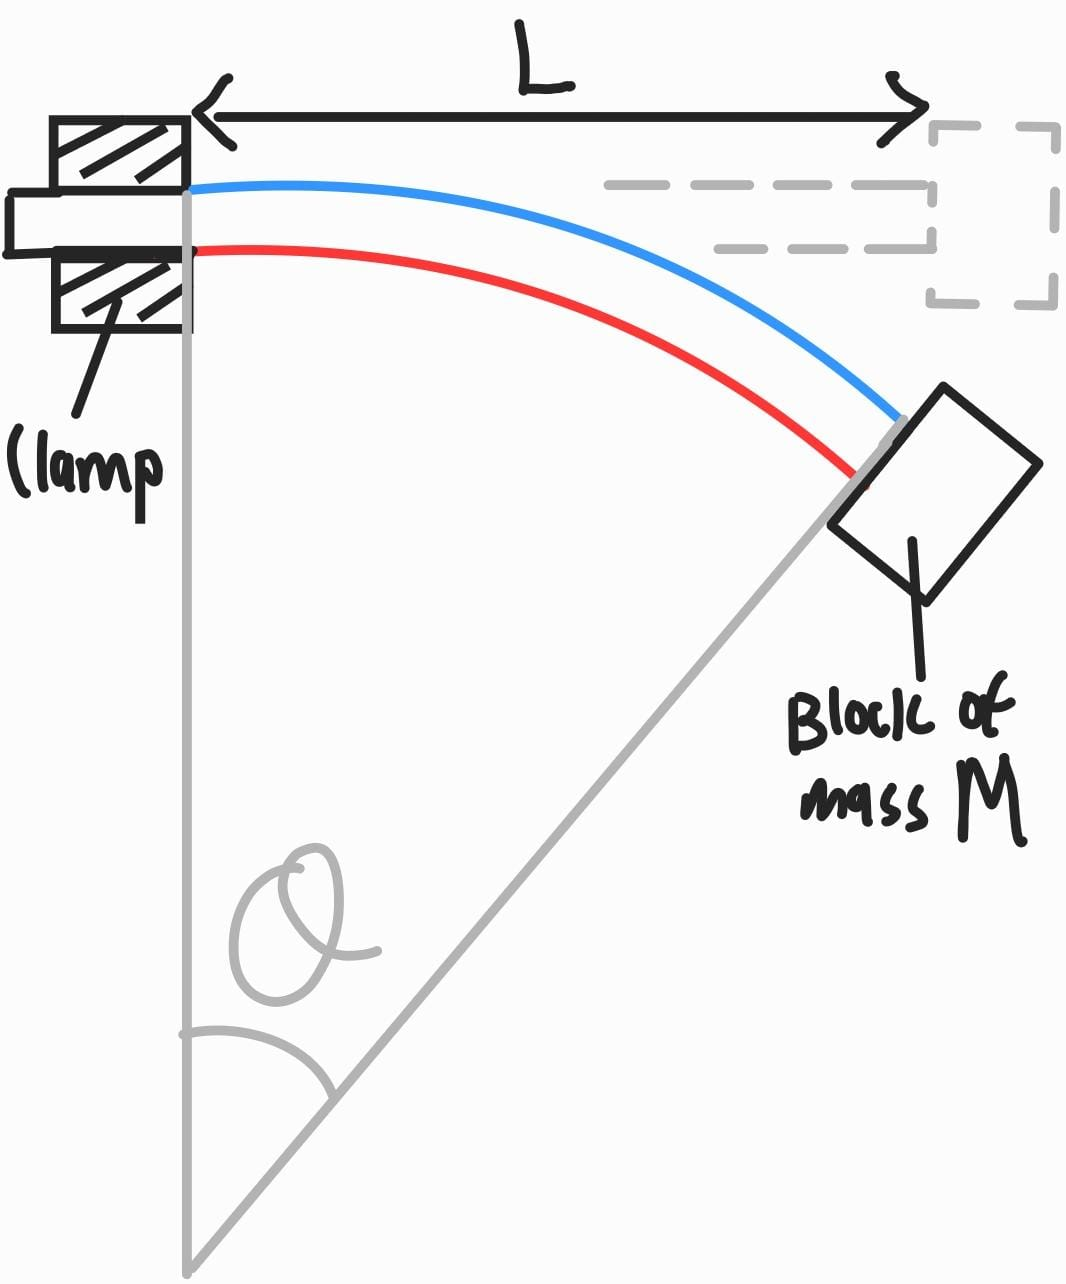
\includegraphics[width=0.3\textwidth]{../images/strip-compession-extension.jpg}
        \caption{\ref{Me}}
        \label{fig:strip-compression-extension}
    \end{figure}
    Explain why the part of the strip is compressed and part of the strip is extended. \hspace*{\fill} [3]
    \begin{itemize}[label={--}]
        \item For the bent strip, the upper and lower surfaces form two arcs subtended by the same angle. 
        \item Since the upper surface has a larger radius of curvature, it is bent longer than \(L\); it is extended.
        \item Since the lower surface has a shorter radius of curvature, it is bent shorter than \(L\); it is compressed.  
    \end{itemize}
    \footnotetext{Each school's solution has a different answer to this question. So, its hard to know what exactly is required. I just picked the one that seems the most value-adding --- i.e. does not just subtly paraphrase the question.}
\end{example}